En este capítulo desarrollamos un estudio sistemático de la opacidad de neutrinos para distintas condiciones termodinámicas para evaluar el impacto que tiene la estructura que se forma.
Estudiamos la opacidad de neutrinos de la materia heterogénea a distintas condiciones termodinámicas para distintas densidades, fracciones de protones y temperatura, calculando la opacidad del muy largo rango y la distribución de fragmentos.
La opacidad de los neutrinos es de crucial importancia para la evolución térmica de las supernovas y el scattering de neutrinos.

\section{Introducción}\label{sc:intro}
\todo[inline]{Acá va la introducción a los reconocedores de fragmentos.
Además, tendría que haber un apéndice a posteriori.}

\section{Clusters}\label{sc:clusters}

\begin{figure*}[H,floatfix]  \centering
  \begin{subfigure}[h!]{0.40\columnwidth}
    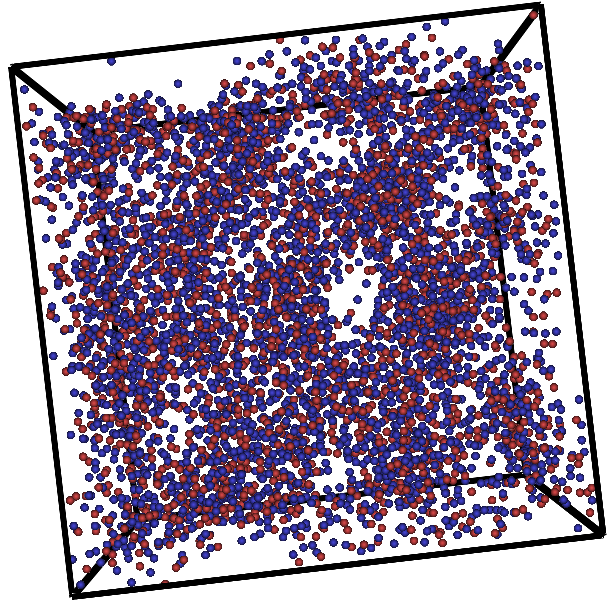
\includegraphics[width=\columnwidth]{nuevas_pastas/x04-d005-T05.png}
    \caption{$x=0.4,\, T=0.5\,\text{MeV}$}
    \label{subfig:04-05}
  \end{subfigure}
  \begin{subfigure}[h!]{0.40\columnwidth}
    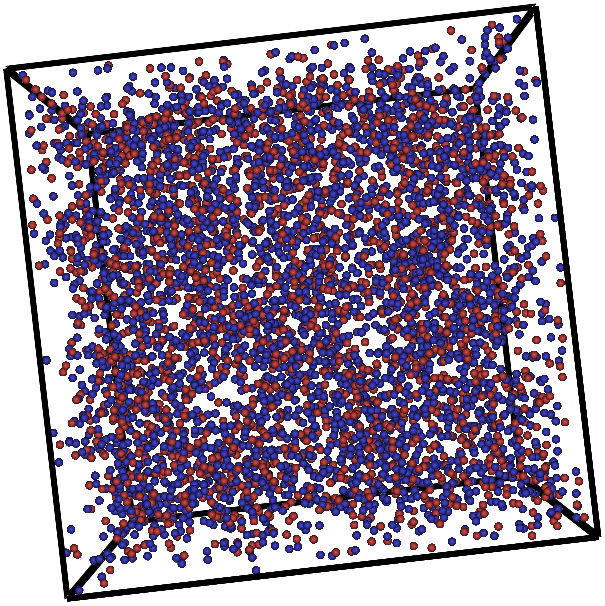
\includegraphics[width=\columnwidth]{nuevas_pastas/x04-d005-T10.png}
    \caption{$x=0.4,\, T=1.0\,\text{MeV}$}
    \label{subfig:04-10}
  \end{subfigure}
  \begin{subfigure}[h!]{0.40\columnwidth}
    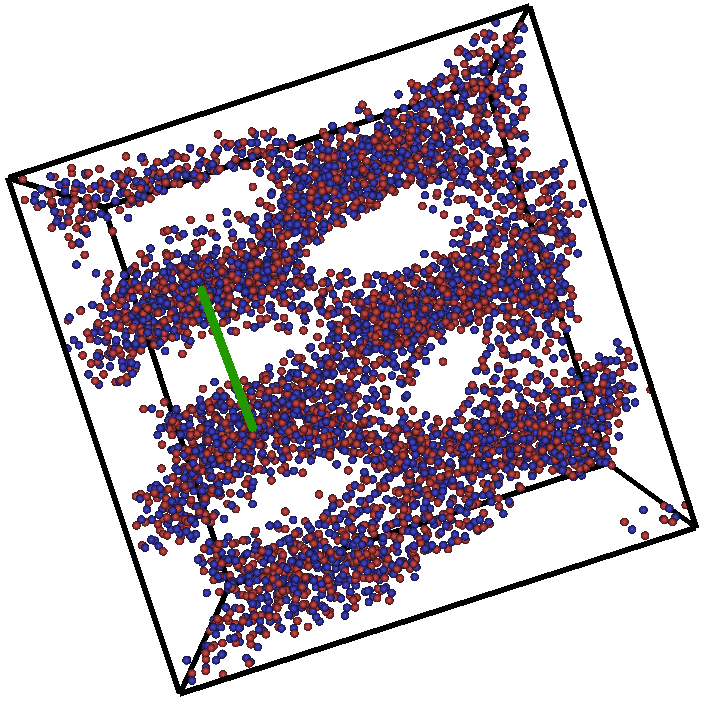
\includegraphics[width=\columnwidth]{nuevas_pastas/x05-d005-T05.png}
    \caption{$x=0.5,\, T=0.5\,\text{MeV}$}
    \label{subfig:05-05}
  \end{subfigure}
  \begin{subfigure}[h!]{0.40\columnwidth}
    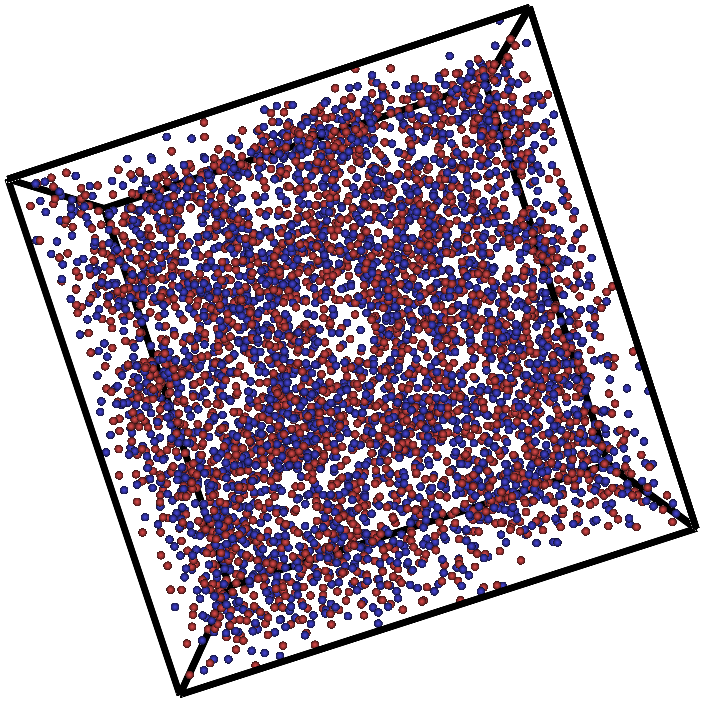
\includegraphics[width=\columnwidth]{nuevas_pastas/x05-d005-T10.png}
    \caption{$x=0.5,\, T=1.0\,\text{MeV}$}
    \label{subfig:05-10}
  \end{subfigure}
  \caption{Estructuras del sistema con densidad $\rho = 0.04\,\text{fm}^{-3}$ para distintos valores de fracción de protones y temperatura.
    Las estructuras obtenidas a $T=0.5\,\text{MeV}$ difieren considerablemente.
    Sin embargo, ambas muestran inhomogeneidades.
    Podemos ver en el panel~\ref{subfig:05-05} una línea verde que marca la longitud de $\approx 15\,\text{fm}$.}
  \label{fig:morpho}
\end{figure*}

En la figura~\ref{fig:morpho} mostramos cuatro estructuras distintas para fracción de protones de $x=0.4$ y $x=0.5$, y temperatura $T=0.5\,\text{MeV}$ y $T=1.0\,\text{MeV}$.
Claramente podemos ver que las estructuras ya no se limitan a las que originalmente propusieron Ravenhall \emph{et al.}~\cite{ravenhall_structure_1983}.
Para estudiarlas en mayor profundidad, podemos ver en la figura~\ref{fig:cluster} la distribución de fragmentos correspondiente al algoritmo MSTE.\@
En esta figura podemos ver que para una fracción de protones de $x=0.2$ hay muchos nucleones aislados que son casi exclusivamente neutrones.
Éstos funcionan como un gas de neutrones en el que se embebe la estructura de protones subyacente.

\begin{figure*}  \centering
  \begin{subfigure}[h!]{0.4\columnwidth}
    \includegraphics[width=\columnwidth]{nuevas_pastas/{{mste_0.2_0.04_2.0}}}
    \caption{$x=0.2$}
  \end{subfigure}
  \begin{subfigure}[h!]{0.4\columnwidth}
    \includegraphics[width=\columnwidth]{nuevas_pastas/{{mste_0.3_0.04_2.0}}}
    \caption{$x=0.3$}
  \end{subfigure}
  \begin{subfigure}[h!]{0.4\columnwidth}
    \includegraphics[width=\columnwidth]{nuevas_pastas/{{mste_0.4_0.04_2.0}}}
    \caption{$x=0.4$}
  \end{subfigure}
  \begin{subfigure}[h!]{0.4\columnwidth}
    \includegraphics[width=\columnwidth]{nuevas_pastas/{{mste_0.5_0.04_2.0}}}
    \caption{$x=0.5$}
  \end{subfigure}
  \caption{Distribución de fragmentos para el algoritmo MSTE para temperatura $T = 2.0\,\text{MeV}$, densidad $\rho = 0.04\,\text{fm}^{-3}$ y diferentes fracciones de protones.
    Para la fracción de protones más baja de las estudiadas, $x = 0.2$, el cluster grande tiene una fracción de protones mayor (aproximadamente $30\%$ más alta) y hay muchos neutrones aislados.
    Notar que las escalas son distintas para cada gráfico.}
  \label{fig:cluster}
\end{figure*}

Otra consecuencia del gas de neutrones es que la fracción de protones de la estructura de pasta generalizada es ligeramente mayor que la fracción de protones original del sistema simulado.
Podemos ver de la figura~\ref{fig:cluster} que la fracción de protones en el fragmento grande es de alrededor de $x = 0.25$, mientras que la fracción de protones macroscópica es $x = 0.2$.
En la figura~\ref{fig:large_mass} podemos observar la masa del fragmento máas grande.
Se puede ver que incluso para temperaturas muy altas ($T = 2.0\,\text{MeV}$) aparece un fragmento muy grande para todas las fracciones de protones.
Todos los fragmentos más grandes contienen más del $50\%$ de la masa total del sistema.

\begin{figure}
  \centering
  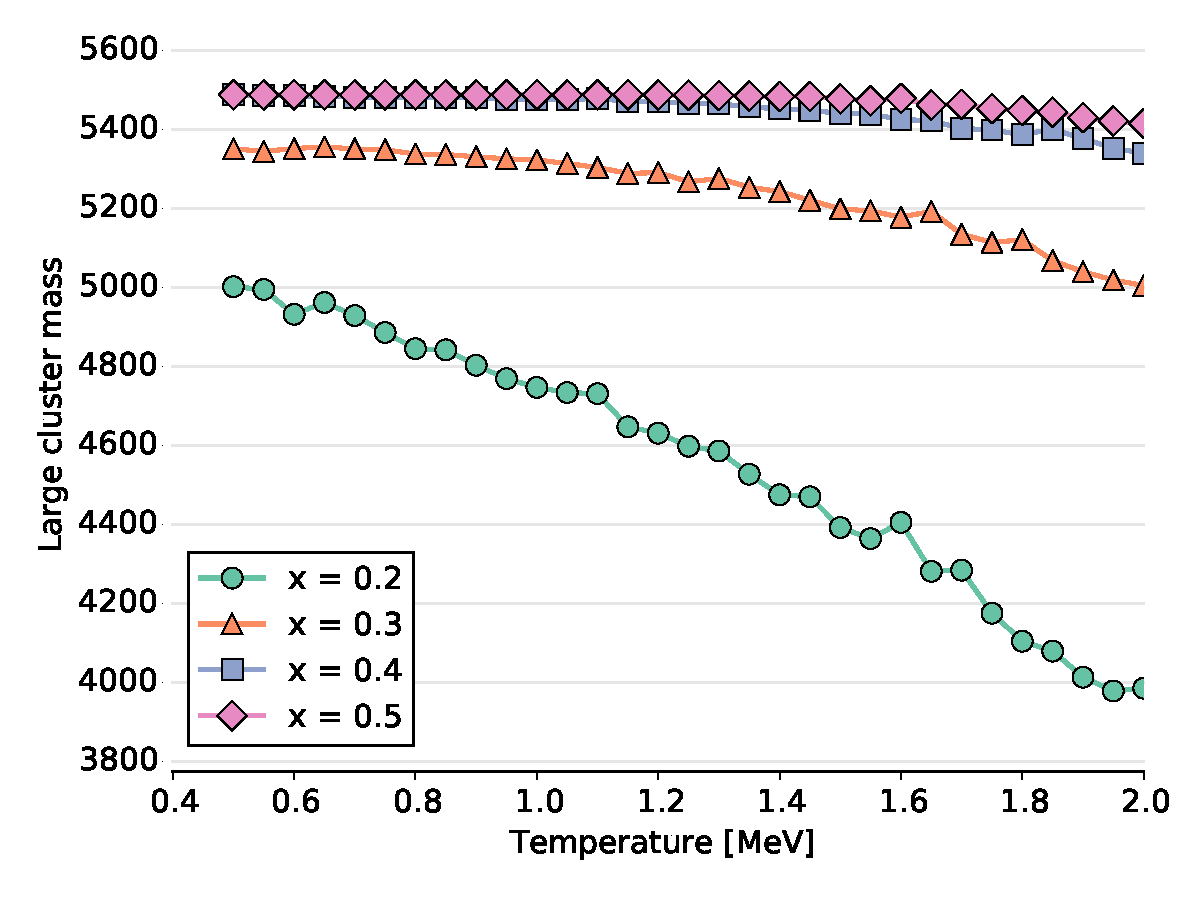
\includegraphics[width=0.4\columnwidth]{nuevas_pastas/large_mass}
  \caption{Masa del fragmento más grande para $\rho = 0.04\,\text{fm}^{-3}$ para distintos valores de $x$.}
  \label{fig:large_mass}
\end{figure}

\section{Opacidad de neutrinos}\label{sc:opacity}

Las figuras~\ref{fig:gr_sq} y~\ref{fig:gr_sq_gnocchi} muestran la función distribución de pares y el factor de estructura \todo[inline]{ver apéndice para una explicación detallada del cálculo} para las fases de \emph{lasagna} y \emph{gnocchi} --- ver epígrafe para más detalles.
En la función de distribución de pares podemos identificar (marcado con $\color{green} \blacktriangledown$) el pico que pertenece a la estructura cristalina de los neutrones dentro de la pasta (correlación con los vecinos más cercanos) y también una correlación de muy largo rango (marcada con una línea discontinua $\color{red}-\,-$.);
este rango es el que genera el pico para los bajos momentos en el factor de estructura, relacionado con las estructuras de tipo pasta.
El factor de estructura muestra un pico en $q_\text{peak} = 0.43\,\text{fm}^{-1}$ para la \emph{lasagna} y $q_\text{peak} = 0.37\,\text{fm}^{-1}$ para los \emph{gnocchi}, con un ancho de alrededor de
$\text{FWHM} = 0.08\,\text{fm}^{-1}$, definiendo un rango de longitudes de onda en las que la estructura es considerablemente opaca.

\begin{figure}  \centering
  \begin{subfigure}[h!]{0.4\columnwidth}
    \centering
    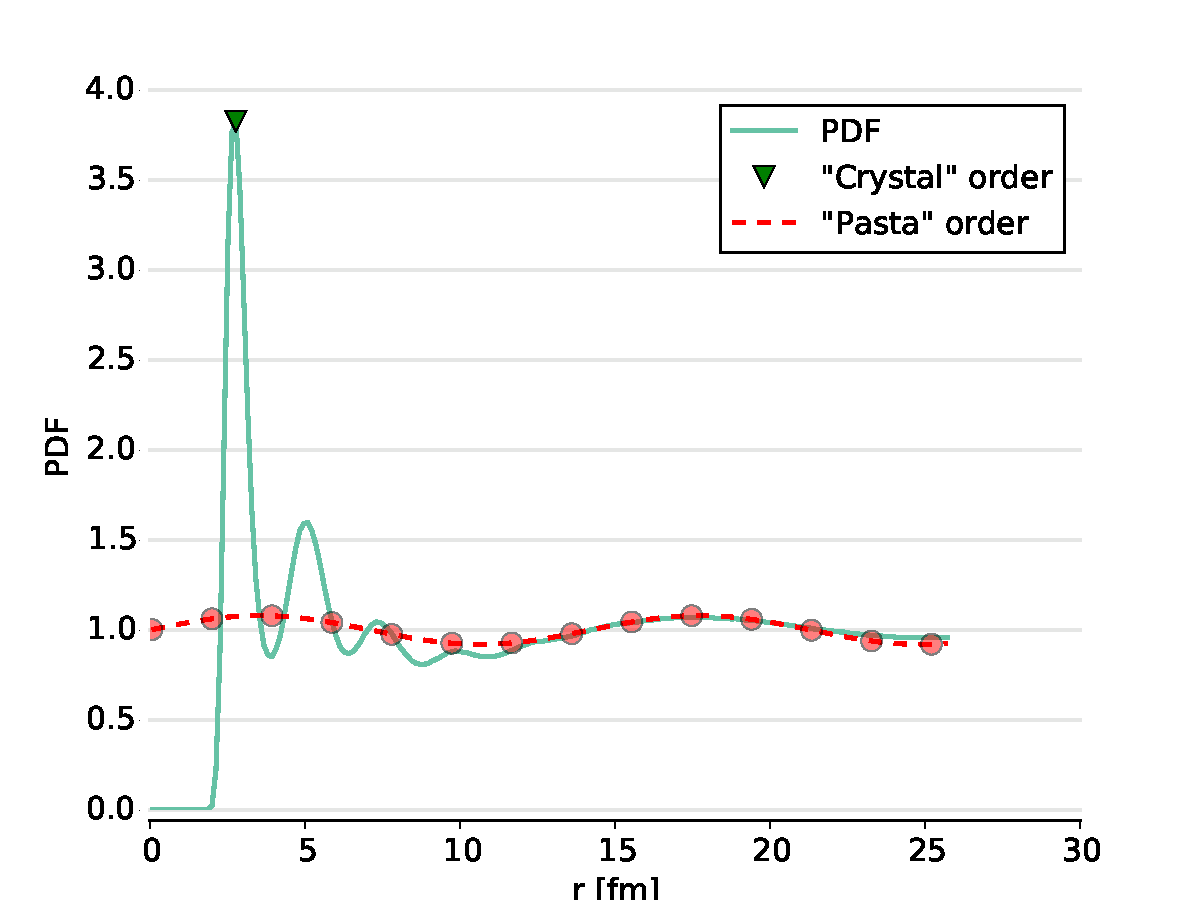
\includegraphics[width=\columnwidth]{nuevas_pastas/rdf}
    \caption{Función de distribución de pares.}
      \label{sfig:gr}
  \end{subfigure}
  \begin{subfigure}[h!]{0.4\columnwidth}
    \centering
    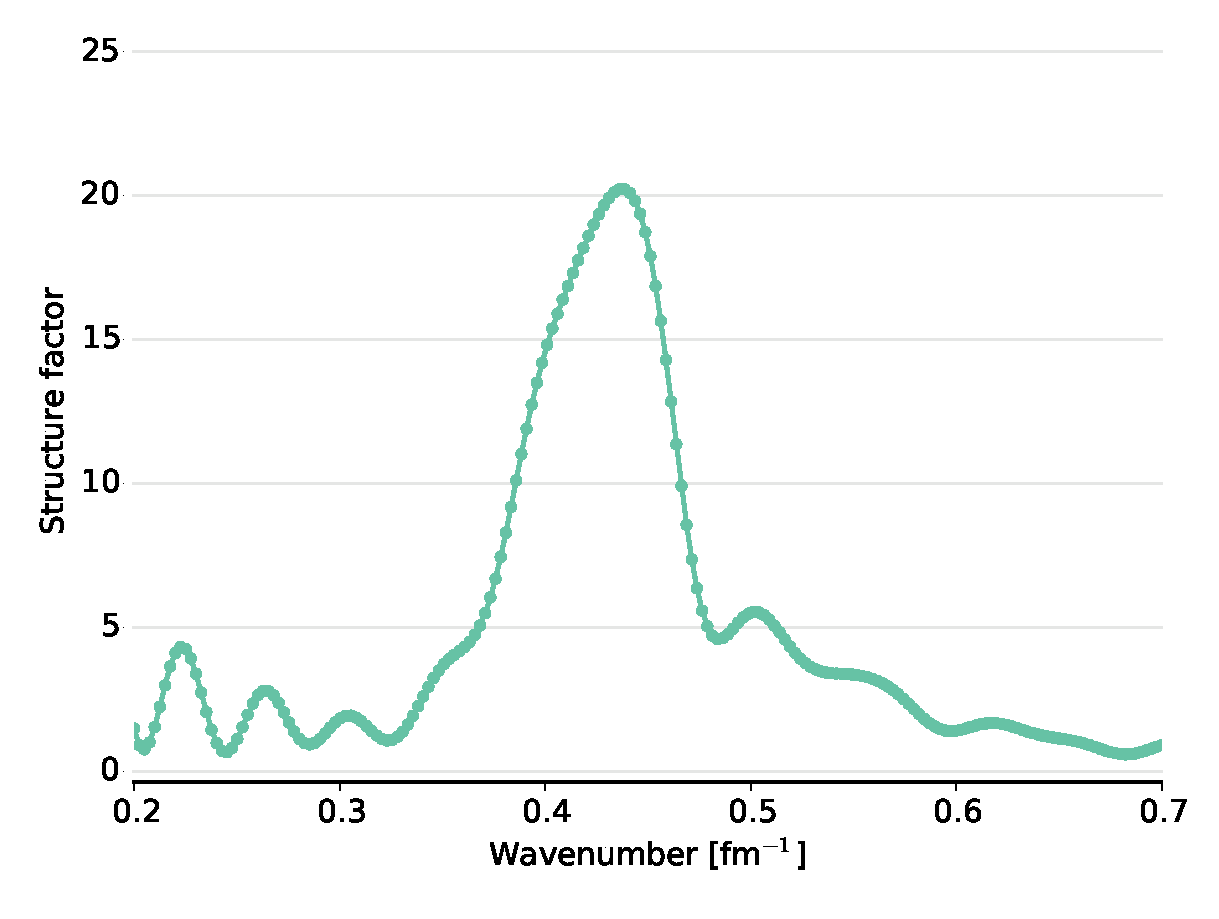
\includegraphics[width=\columnwidth]{nuevas_pastas/ssf}
    \caption{Factor de estructura.}
      \label{sfig:ssf}
  \end{subfigure}
  \caption{\ref{sfig:gr} Función de distribución de pares y ~\ref{sfig:ssf} factor de estructura para un sistema con fracción de protones $x=0.4$, densidad $\rho=0.04\,\text{fm}^{-3}$ y temperatura $T=0.5\,\text{MeV}$.
    El primer pico en $g(r)$, debido a las estructuras cristalinas, está marcado con $\color{green} \blacktriangledown$, mientras que el rango muy largo está marcado con una línea discontinua $\color{red}-\,-$.
    En el factor de estructura podemos ver el pico en $q_\text{peak} = 0.43\,\text{fm}^{-1}$ con un ancho de alrededor de $\text{FWHM} = 0.08\,\text{fm}^{-1}$.
    Las ``ondas'' para los bajos momentos se deben a efectos de tamaño finito.}
  \label{fig:gr_sq}
\end{figure}

\begin{figure}  \centering
  \begin{subfigure}[h!]{0.4\columnwidth}
    \centering
    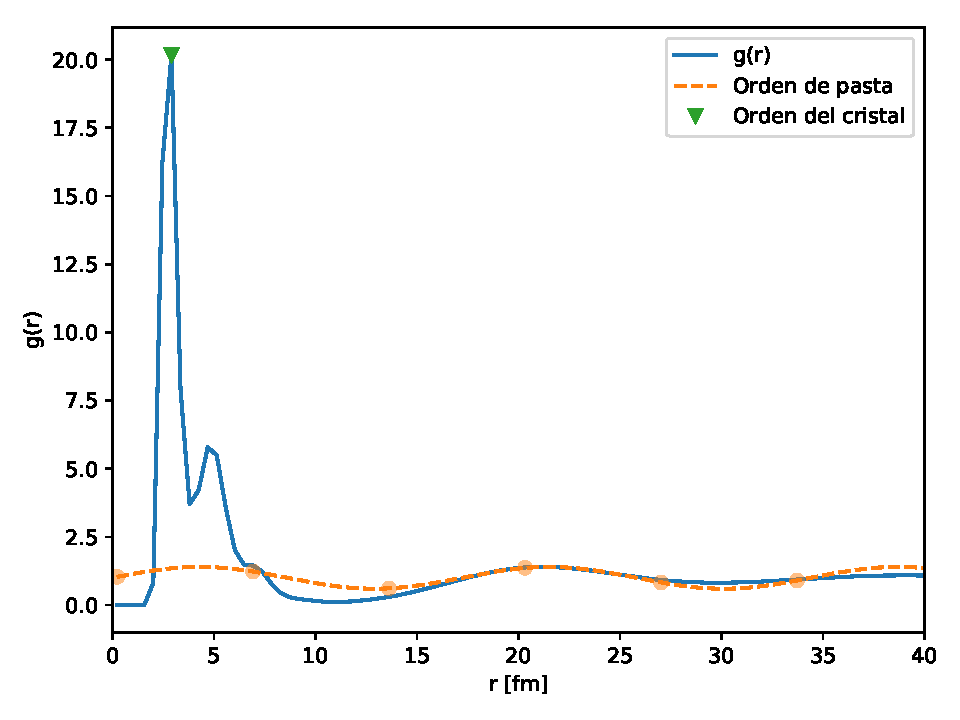
\includegraphics[width=\columnwidth]{nuevas_pastas/rdf_gnocchi}
    \caption{Función de distribución de pares.}
      \label{sfig:gr_gnocchi}
  \end{subfigure}
  \begin{subfigure}[h!]{0.4\columnwidth}
    \centering
    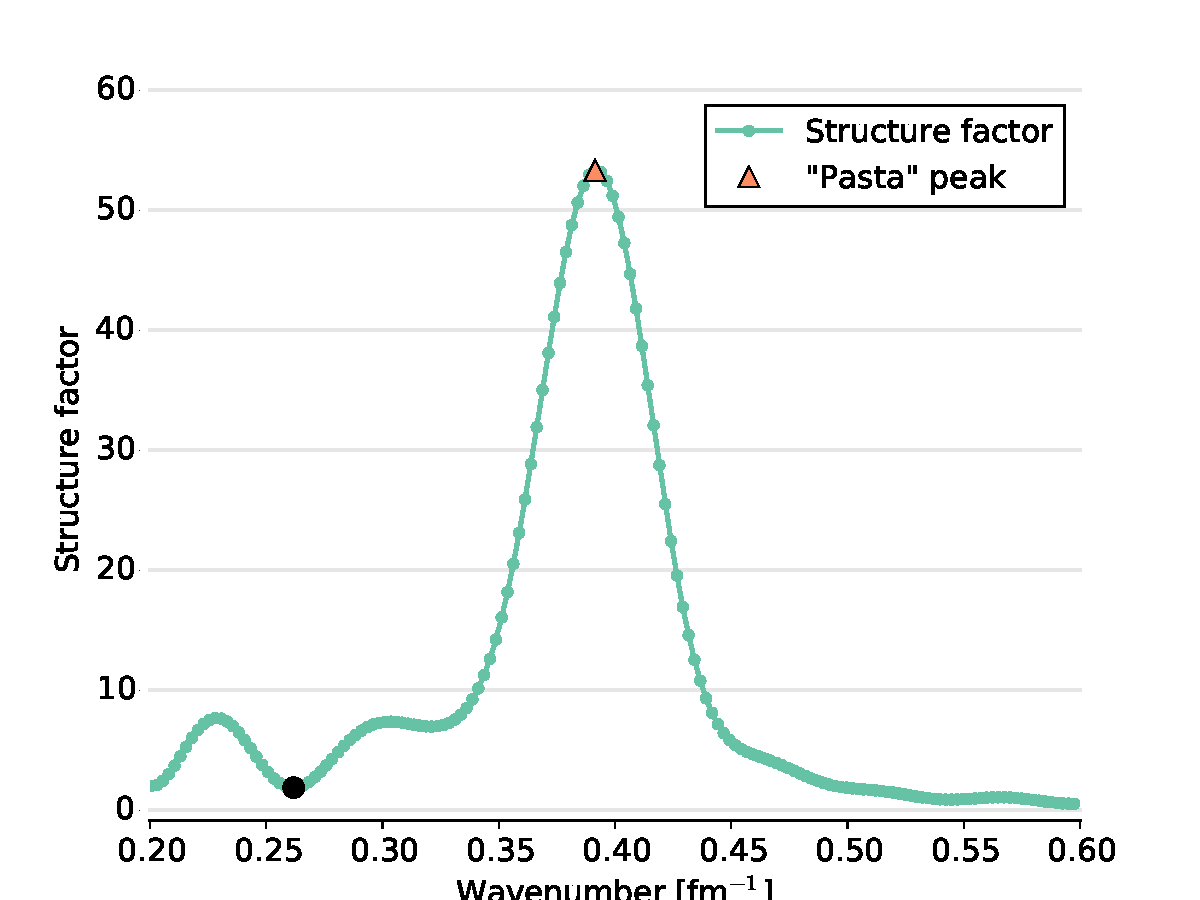
\includegraphics[width=\columnwidth]{nuevas_pastas/ssf_gnocchi}
    \caption{Factor de estructura.}
      \label{sfig:ssf_gnocchi}
  \end{subfigure}
  \caption{~\ref{sfig:gr_gnocchi} Función de distribución de pares y~\ref{sfig:ssf} factor de estructura para un sistema con fracción de protones $x=0.4$, densidad $\rho=0.01\,\text{fm}^{-3}$ y temperatura $T=0.5\,\text{MeV}$.
    Como en la figura~\ref{fig:gr_sq}, podemos ver la estructura cristalina y de pasta en la función de distribución de pares, así como el pico de la pasta en el factor de estructura.
    Este pico está localizado en $q_\text{peak} = 0.37\,\text{fm}^{-1}$ con un ancho de alrededor de $\text{FWHM} = 0.08\,\text{fm}^{-1}$.
    Las ``ondas'' para los bajos momentos se deben a efectos de tamaño finito.}
  \label{fig:gr_sq_gnocchi}
\end{figure}


Para cada configuración de fracción de protones, densidad y temperatura, calculamos el factor de estructura y extraemos su pico para momentos bajos.
Llamaremos a este valor \emph{pico de opacidad}.

Simulamos el sistema para un total de aproximadamente 1000 configuraciones distintas (4 fracciones de protones, 10 densidads y 30 tempretaruas).
Para cada combinación $(x, \rho, T)$ calculamos la función de distribución de pares, cuya transformada de Fourier es el factor de estructura.
De este factor de estructura obtenemos el pico de opacidad.
Un detalle a considerar es que, como mencionamos en el capítulo~\ref{ch:transicion}, debajo de cierta temperatura (cercana a $1\,\text{MeV}$) el sistema puede \todo[inline]{congelarse} en uno de los muchos mínimos locales.
Es debido a esto que el sistema no puede ser simulado directamente a temperaturas bajas.
En cambio, las temperaturas bajas deben ser obtenidas a partir de temperaturas altas, enfriando cuidadosamente el sistema y garantizando su termalización, tratando de simular así una sucesión de estados de equilibrio.

La figura~\ref{fig:low_t} muestra la longitud de onda y la altura del \emph{pico de opacidad} para la temperatura más baja estudiada en este trabajo ($T = 0.5\,\text{MeV}$) como función de la densidad.
Podemos observar que la longitud de onda decrece a medida que aumenta la densidad, implicando que la longitud de correlación de la estructura es cada vez menor.
Esto es de esperar, ya que cuanto mayor la densidad, más cercanas están las estrucutras.
Sin embargo, queremos enfatizar en que la estructura cambia con la densidad no sólo con transiciones en la morfología (por ejemplo de \emph{spaghetti} a \emph{lasagna}) sino también, por ejemplo, con fragmentos de \emph{gnocchi} que tienen distintos tamaños para distintas densidades.
Esta combinación entre el cambio de estructuras y el cambio de la distribución espacial para cada estructura resulta en la figura ~\ref{sfig:wl}.
Podemos ver que la longitud de onda para máxima opacidad cambia rápidamente para densidades bajas (los \emph{gnocchi}), pero tiende a estabilizarse para las otras pastas.
Se debe considerar también que, ya que $S(q)$ tiene un cierto ancho cerca del pico, la estructura \todo[inline]{dispersaría} neutrinos en un rango de longitudes de onda cercanas a dicho máximo
Es interesante notar que la altura del \emph{pico de opacidad} toma su máximo valor para $\rho = 0.01\,\text{fm}^{-3}$, donde aún tenemos \emph{gnocchi}, como se puede ver por la distribución de fragmentos en la figura~\ref{fig:cluster_gnocchi}.

\begin{figure}  \centering
  \begin{subfigure}[h!]{0.4\columnwidth}
    \includegraphics[width=\columnwidth]{nuevas_pastas/{{lambda_density}}}
    \caption{Longitud de onda del pico de opacidad}
    \label{sfig:wl}
  \end{subfigure}
  \begin{subfigure}[h!]{0.4\columnwidth}
    \includegraphics[width=\columnwidth]{nuevas_pastas/{{height_density}}}
    \caption{Altura del pico de opacidad}
    \label{sfig:ht}
  \end{subfigure}
  \caption{\ref{sfig:wl} Longitud de onda y~\ref{sfig:ht} altura del pico de opacidad para temperaturas bajas ($T = 0.5\,\text{MeV}$) como función de la densidad para distintas fracciones de protones.
    Podemos observar que la longitud de onda cambia rápidamente para $\rho < 0.02\,\text{fm}^{-3}$ (fase \emph{gnocchi}) y se estabiliza para densidades más altas.}
  \label{fig:low_t}
\end{figure}

\begin{figure*}  \centering
  \begin{subfigure}[h!]{0.4\columnwidth}
    \includegraphics[width=\columnwidth]{nuevas_pastas/{{mste_0.2_0.01_0.5}}}
    \caption{$x=0.2$}
  \end{subfigure}
  \begin{subfigure}[h!]{0.4\columnwidth}
    \includegraphics[width=\columnwidth]{nuevas_pastas/{{mste_0.3_0.01_0.5}}}
    \caption{$x=0.3$}
  \end{subfigure}
  \begin{subfigure}[h!]{0.4\columnwidth}
    \includegraphics[width=\columnwidth]{nuevas_pastas/{{mste_0.4_0.01_0.5}}}
    \caption{$x=0.4$}
  \end{subfigure}
  \begin{subfigure}[h!]{0.4\columnwidth}
    \includegraphics[width=\columnwidth]{nuevas_pastas/{{mste_0.5_0.01_0.5}}}
    \caption{$x=0.5$}
  \end{subfigure}
  \caption{Distribución de fragmentos con el algoritmo MSTE para temperatura $T = 0.5\,\text{MeV}$, densidad $\rho = 0.01\,\text{fm}^{-3}$ y distintas fracciones de protones.
    Podemos ver que todas tienen distribuciones de masa tipo \emph{gnocchi}.
    Notar que las escalas son distintas para cada gráfico.}
  \label{fig:cluster_gnocchi}
\end{figure*}


En la figura~\ref{fig:absorption} mostramos el \emph{pico de opacidad} para las distintas configuraciones termodinámicas.
Podemos ver que a medida que decrece la fracción de protones, también decrece la opacidad.
Para cada fracción de protones estudiada, la altura del pico de opacidad decae rápidamente para temperaturas mayores a $T=0.8\,\text{MeV}$, y es aproximadamente $1/4$ de la altura del pico de opacidad para $T=0.5\,\text{MeV}$.
La opacidad del sistema decrece a medida que se reduce la fracción de protones porque la estructura del sistema se debe a la interacción de rango largo de Coulomb entre protones.
Cuando hay sólo un proton por neutrón ($x = 0.5$), la estructura de neutrones sigue casi idénticamente la de los protones.
Sin embargo, a medida que la proporción de neutrones aumenta, la estructura de neutrones se difumina y su correlación de muy largo rango empieza a desaparecer.
Este efecto puede verse en la distribución de fragmentos para $x = 0.2$, donde tenemos muchos neutrones aislados, que forman el gas de neutrones.
Estas características afectan las inhomogeneidades que aparecen en $x = 0.5$, suprimiendo su opacidad de muy largo rango.

\begin{figure*}  \centering
  \begin{subfigure}[h!]{0.4\columnwidth}
    \centering
    \includegraphics[width=\columnwidth]{nuevas_pastas/{{s_0.2}}}
    \caption{$x=0.2$}
  \end{subfigure}
  \begin{subfigure}[h!]{0.4\columnwidth}
    \centering
    \includegraphics[width=\columnwidth]{nuevas_pastas/{{s_0.3}}}
    \caption{$x=0.3$}
  \end{subfigure}
  \begin{subfigure}[h!]{0.4\columnwidth}
    \centering
    \includegraphics[width=\columnwidth]{nuevas_pastas/{{s_0.4}}}
    \caption{$x=0.4$}
  \end{subfigure}
  \begin{subfigure}[h!]{0.4\columnwidth}
    \centering
    \includegraphics[width=\columnwidth]{nuevas_pastas/{{s_0.5}}}
    \caption{$x=0.5$}
  \end{subfigure}
  \caption{Pico de opacidad para el rango muy largo para distintas fracciones de protones como función de la temperatura y la densidad.
    Podemos ver que la opacidad decrece drásticamente para $T \gtrsim 0.8\,\text{MeV}$.
    También mostramos aquí que la opacidad se ve afectada por la fracción de protones, como se puede notar por las escalas en la barra de colores de cada gráfico.
    Se puede notar que en la opacidad para  $x = 0.2$ y $x = 0.3$, los resultados son en mayor parte ruido.}
  \label{fig:absorption}
\end{figure*}

De la figura~\ref{fig:large_mass} podemos ver que incluso para altas temperaturas ($T = 2.0\,\text{MeV}$) aparece un fragmento grande para todas las fracciones de protones.
Este fragmento grande es la estructura que llamamos \emph{Pasta Nuclear Generalizada}, responsable de la interacción de largo rango.
La razón por la que la opacidad se deprime drásticamente a medida que la temperatura aumenta, en conclusión, no es porque desaparezca la estructura del fragmento grande, sino debido a cambios dentro de ella.

\section{Conclusiones}\label{sc:conc}

La materia rica en neutrones desarrolla estructuras no homogéneas (usualmente conocidas como pasta nuclear) que alteran considerablemente su opacidad a neutrinos.
Analizando el comportamiento del factur de estructura de neutrón-neutrón y la función de distribución de pares para un gran rango de densidades, temperaturas y fracción de protones, podemos calcular la longitud de onda para la cual se produce el máximo \emph{scattering}.
Vimos que para altas densidades, donde esperamos que aparezcan fragmentos muy grandes (\emph{spaghetti} u \emph{lasagna}), la longitud de onda del pico de opacidad se mantiene relativamente constante, y la máxima opacidad se obtiene para neutrinos muy energéticos ($E_\nu \approx 80\,\text{MeV}$, típicos de una muy inicial etapa de evolución de las proto-estrellas de neutrones).
A medida que disminuye la densidad, nos movemos hacia la fase de \emph{gnocchi}, en la cual los fragmentos son de tamaño finito.
Ene ste caso, la máxima opacidad se mueve a energías menores.
Como podemos ver en la figura~\ref{fig:absorption}, este aumento en la opacidad no sólo se produce cuando las heterogeneidades forman parte de las comúnmente conocidas como pasta nuclear, sino también cuando son bastante diferentes (la \emph{pasta nuclear generalizada} que podemos ver en la figura~\ref{fig:morpho}).

Es de esperar que estos resultados sean cualitativamente correctos, pero que dependan cuantitativamente del modelo escogido para describir la materia rica en neutrones.
El modelo que estamos utilizando en este trabajo fue puesto a prueba extensivamente en colisiones y en física de iones pesados; es por esta razón que lo escogimos para describir cuantitativamente la materia rica de neutrones.

\todo[inline]{Los modelos hidrodinámicos para la materia rica en neutrones~\cite{ruffert_coalescing_1995, mezzacappa_investigation_1998, geppert_temperature_2004, woosley_physics_2005, liebendorfer_supernova_2005} pueden sugerir fracciones de protones, densidades y temperaturas para distintas condiciones (supernovas, proto-estrellas de neutrones, estrellas de neutrones).}
De este trabajo podemos encontrar, para este modelo específico, la opacidad a los neutrinos para distintas condiciones termodinámicas.
Consecuentemente, combinando estos dos resultados con mediciones eventuales de la opacidad de los neutrinos en estrellas de neutrones, podemos comprobar la validez de distintos modelos nucleares y, en consecuencia, avanzar hacia la ecuación de estado de la materia nuclear.

\section{El cálculo del factor de estructura}

El factor de estructura de un sistema se define como la \emph{amplitud de scattering}~\cite{egami_underneath_2003}

\begin{equation}
  \Psi(\mathbf{Q}) = \frac{1}{\langle b\rangle} \sum_i b_i
  \text{e}^{i\mathbf{Q}\cdot\mathbf{R}_i}
  \label{eq:scat_amp}
\end{equation}

con $\mathbf{Q}$ el vector de difracción o transferencia de momento.
$\mathbf{R}_i$ es la posición de la partícula $i$, y $\langle b\rangle$ es el promeedio de la amplitud de scattering de cada partícula en el vacío $b_i$.
A partir de este momento, vamos a considerar que todas las partículas son de la misma especie, $b_i = b$.

A partir de $\Psi(\mathbf{Q})$ definimos $S(\mathbf{Q})$ como

\begin{equation*}
  S(\mathbf{Q}) = \frac{1}{N} |\Psi(\mathbf{Q})|^2
\end{equation*}

La conclusión \emph{inmediata} de esta expresión es que el factor de estructura debe ser positivo siempre para todo valor de $\mathbf{Q}$.
Podemos expandir la amplitud de scattering y utilizar $|z|^2 = z\cdot z^*$  y, si todos los átomos son del mismo tipo,


\begin{align*}
  S(\mathbf{Q}) &= \frac{1}{N} \left( \sum_i \text{e}^{i\mathbf{Q}\cdot\mathbf{R}_i} \right)
  \left( \sum_j \text{e}^{-i\mathbf{Q}\cdot\mathbf{R}_j} \right)\\
  &= \frac{1}{N} \sum_{i, j} \text{e}^{i\mathbf{Q}\cdot(\mathbf{R}_i-\mathbf{R}_j)}\\
  &= \frac{1}{N} \left[N + \sum_{i < j}
    \left(\text{e}^{i\mathbf{Q}\cdot(\mathbf{R}_i-\mathbf{R}_j)} +
      \text{e}^{i\mathbf{Q}\cdot(\mathbf{R}_i-\mathbf{R}_j)}\right)\right]\\
  &= 1 + \frac{2}{N}\sum_{i < j}\cos{\mathbf{Q}\cdot\mathbf{R}_{ij}}
\end{align*}

Usualmente estamos interesados en el conocido como \emph{promedio de polvo} del factor de estructura: es decir, el factor de estructura promediado para todas las posibles orientaciones del vector de difracción (ya que en un polvo tenemos muchas estrucutras orientadas al azar).
Calculamos entonces

\begin{equation*}
  S(q) = \frac{1}{4\pi}\int\text{d}\phi\text{d}(\cos\theta) S(\mathbf{Q})
\end{equation*}

Esta integral puede ser calculada fácilmente si colocamos el eje $z$ en la dirección de $\mathbf{Q}$ e integramos rotando las distancias $\mathbf{R}_{ij}$

\begin{align*}
  S(q) &= \frac{1}{4\pi}\int\text{d}\phi\text{d}(\cos\theta)
  \left[1 + 2\sum_{i < j}\cos\left(q\,r_{ij}\,\cos\theta\right)\right]\\
  &= 1 + \frac{1}{2N}\int\text{d}(\cos\theta)
  2\sum_{i < j}\cos\left(q\,r_{ij}\,\cos\theta\right)\\
  &= 1 + \frac{1}{2N} 2 \sum_{i < j} \left.\frac{\sin(q\,r_{ij}u)}{q\,r_{ij}}\right|_{u=-1}^{u=1}\\
  &= 1 + \frac{2}{N} \sum_{i < j}\frac{\sin(q\,r_{ij})}{q\,r_{ij}}
\end{align*}

Esta es la famosa fórmula de Debye y, como es el promedio de una cantidad que es siempre positiva, debe ser siempre positiva.

Uno de los problemas más usuales cuando modelamos y estudiamos sitemas en simulaciones computacionales es que no tenemos \emph{realmente} sistemas infinitos.
Usamos, para emular el comportamiento de sistemas infinitos, condiciones periódicas de contorno (CPC).
Con las condiciones periódicas de contorno utilizamos la convención de la mínima imagen: de todas las posiciones posibles a través de los contornos para las partículas $i$ and $j$, escogemos el par más cercano.
Utilizando este método para un caso de prueba muy simple (una red cúbica simple tridimensional con 4x4x4=64 partículas) calculamos el factor de estructura que se puede ver en la figura~\ref{fig:ssf_comp}.

\begin{figure}
  \centering
  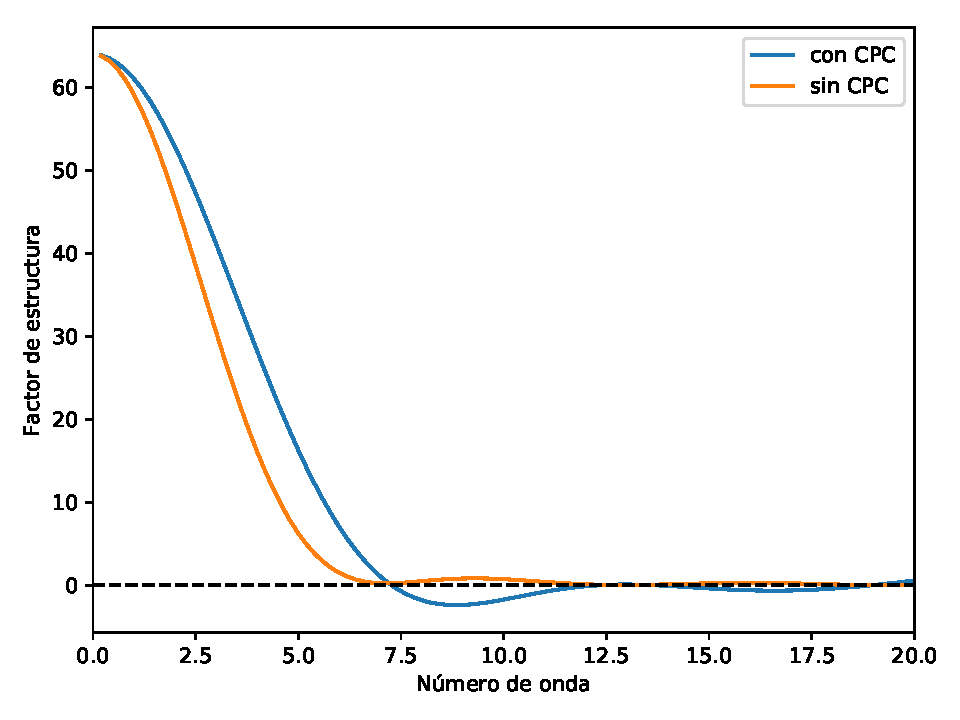
\includegraphics[width=0.4\columnwidth]{nuevas_pastas/ssf_comp.pdf}
  \caption{Comparación del factor de estructura con y sin CPC.
    Es evidente que el factor de estructura calculado con CPC muestra valores negativos, que no deberían existir desde la misma definición del factor de estructura.}
  \label{fig:ssf_comp}
\end{figure}

Podemos ver que el factor de estructura calculado con CPC genera valures negativos, a pesar de que estos valores deberían estar prohibidos.
La razón por la que esto sucede es la convención de mínima imagen: la distancia entre los pares ahroa no es siempre $r_{ij} = r_j - r_i$, sino que depende de si utilizamos las particulas originales o sus imágenes.
En consecuencia, este ``nuevo'' factor de estrucutra no es el producto de dos complejos conjugados\footnote{Más aún, ahora la parte imaginaria de $S(Q)$ ya no es}.
Para explorar el efecto que tiene la convención de la mínima imagen tiene en el factor de estructura, mostramos una comparación del factor de estructura con y sin condiciones de contorno (es decir, con los 64 átomos en el vacío) en la figura~\ref{fig:ssf_comp}.

Esto muestra que el factor de estructura, cuando utilizamos su definición, \emph{sin la convención de la mínima imagen}, es (como era de esperar) siempre positivo.

La pregunta persiste: ¿cómo podemos simular un medio infinito cuando calculamos factores de estructura?
La primera respuesta es que no es obvio que esto pueda ayudar en un medio realmente infinito, ya que las imágenes periódicas de la celda estarían alineadas en un crista lq ue puede interferir con la estructura dentro de la celda (la que queremos estudiar).
Sin embargo, unas pocas réplicas podrían ser suficientes para borrar considerablemente los efectos de tamaño finito.
Una posibilidad es replicar explícitamente la caja, creando las partículas en las celdas vecinas, multiplicando las originales,
Esto, sin embargo, implica un calculo mucho más difícil, ya que la suma para calcular la función de distribución de pares es sobre $N^2$ particles, y replciarla sólo una celda a la derecha y a la izquierda en cada dirección implicaría un tiempo computacional de  $(3^3\cdot N)^2 \approx 700\cdot N^2$.
En general, la complejidad $\mathcal{O}(N^2)$ hace que el cálculo del factor de estructura sea muy costoso para sistemas grandes.

Hay una alternativa para agregar las condiciones de contorno.
Comenzamos con la definición de la \emph{amplitud de scattering} como en~\ref{eq:scat_amp}, pero escribiendo explícitamente las imágenes que queremos considerar:
\begin{equation}
  \Psi(\mathbf{Q}) = \sum_i \sum_j
  \text{e}^{i\mathbf{Q}\cdot(\mathbf{R}_i+\mathbf{\Delta L}_j})
\end{equation}
donde $\mathbf{\Delta L}_j$ es la distancia entre una partícula y su réplica
$j$-ésima. Como las sumas son independientes, podemos escribir:
\begin{equation}
  \Psi(\mathbf{Q}) = \left(\sum_i
    \text{e}^{i\mathbf{Q}\cdot\mathbf{R}_i}\right)
  \left(\sum_j\text{e}^{i\mathbf{Q}\cdot\mathbf{\Delta L}_j}\right)
\end{equation}

Multiplicando por el conjugado, obtenemos el factor de estructura
\begin{align}
  S(\mathbf{Q}) &= \left|\sum_i
    \text{e}^{i\mathbf{Q}\cdot\mathbf{R}_i}\right|^2 \left|\sum_j
    \text{e}^{i\mathbf{Q}\cdot\mathbf{\Delta L}_j}\right|^2\\
  &= S_{\text{cell}}(\mathbf{Q})\,S_{\text{PBC}}(\mathbf{Q})
\end{align}

La ventaja de este cálculo es que es lineal en la suma del número de partículas y el número de répicas que consideremos, $\mathcal{O}(N+M)$, mucho menor que el previo $\mathcal{O}(N^2M^2)$.
En consecuencia, si queremos concentranos en una región de $\mathbf{Q}$, este nuevo enfoque será útil\footnote{Consideremos que con este método necesitamos $\mathcal{O}(N+M)$ cálulos para cada $\mathbf{Q}$, así que no podemos utilizarlo para barrer todo el espectro de $\mathbf{Q}$}.
Quedamos con sólo un datalle, respecto del \emph{powder average}.
No es trivial cómo calcular esta integral, ya que necesitamos darle pesos adecuados a cada ángulo.
En este trabajo utilizamos la cuadratura de Lebedev~\cite{lebedev_values_1975}, aunque otros métodos (como Muestreo por Importancia de Montecarlo) pueden ser útiles en esta situación.